\hypertarget{iii-linear-complexity-rpe-implementation}{%
\subsection{III Linear complexity RPE
implementation}\label{iii-linear-complexity-rpe-implementation}}

In this section we will detail how the relative positional encoding
proposed by \href{https://arxiv.org/abs/1803.02155}{Shaw et al.~(2018)}
can in fact be computed with linear complexity. The \(S_{rel}\) matrix
of scores is computed as
\({S_{rel}}_{ij} = \vec{Q_i} \sdot \vec{RP}_{clip(i-j, -k, k)}\). Here
below the colors represent the index of the query and the number the
index of the relative position.

\begin{figure}
\centering
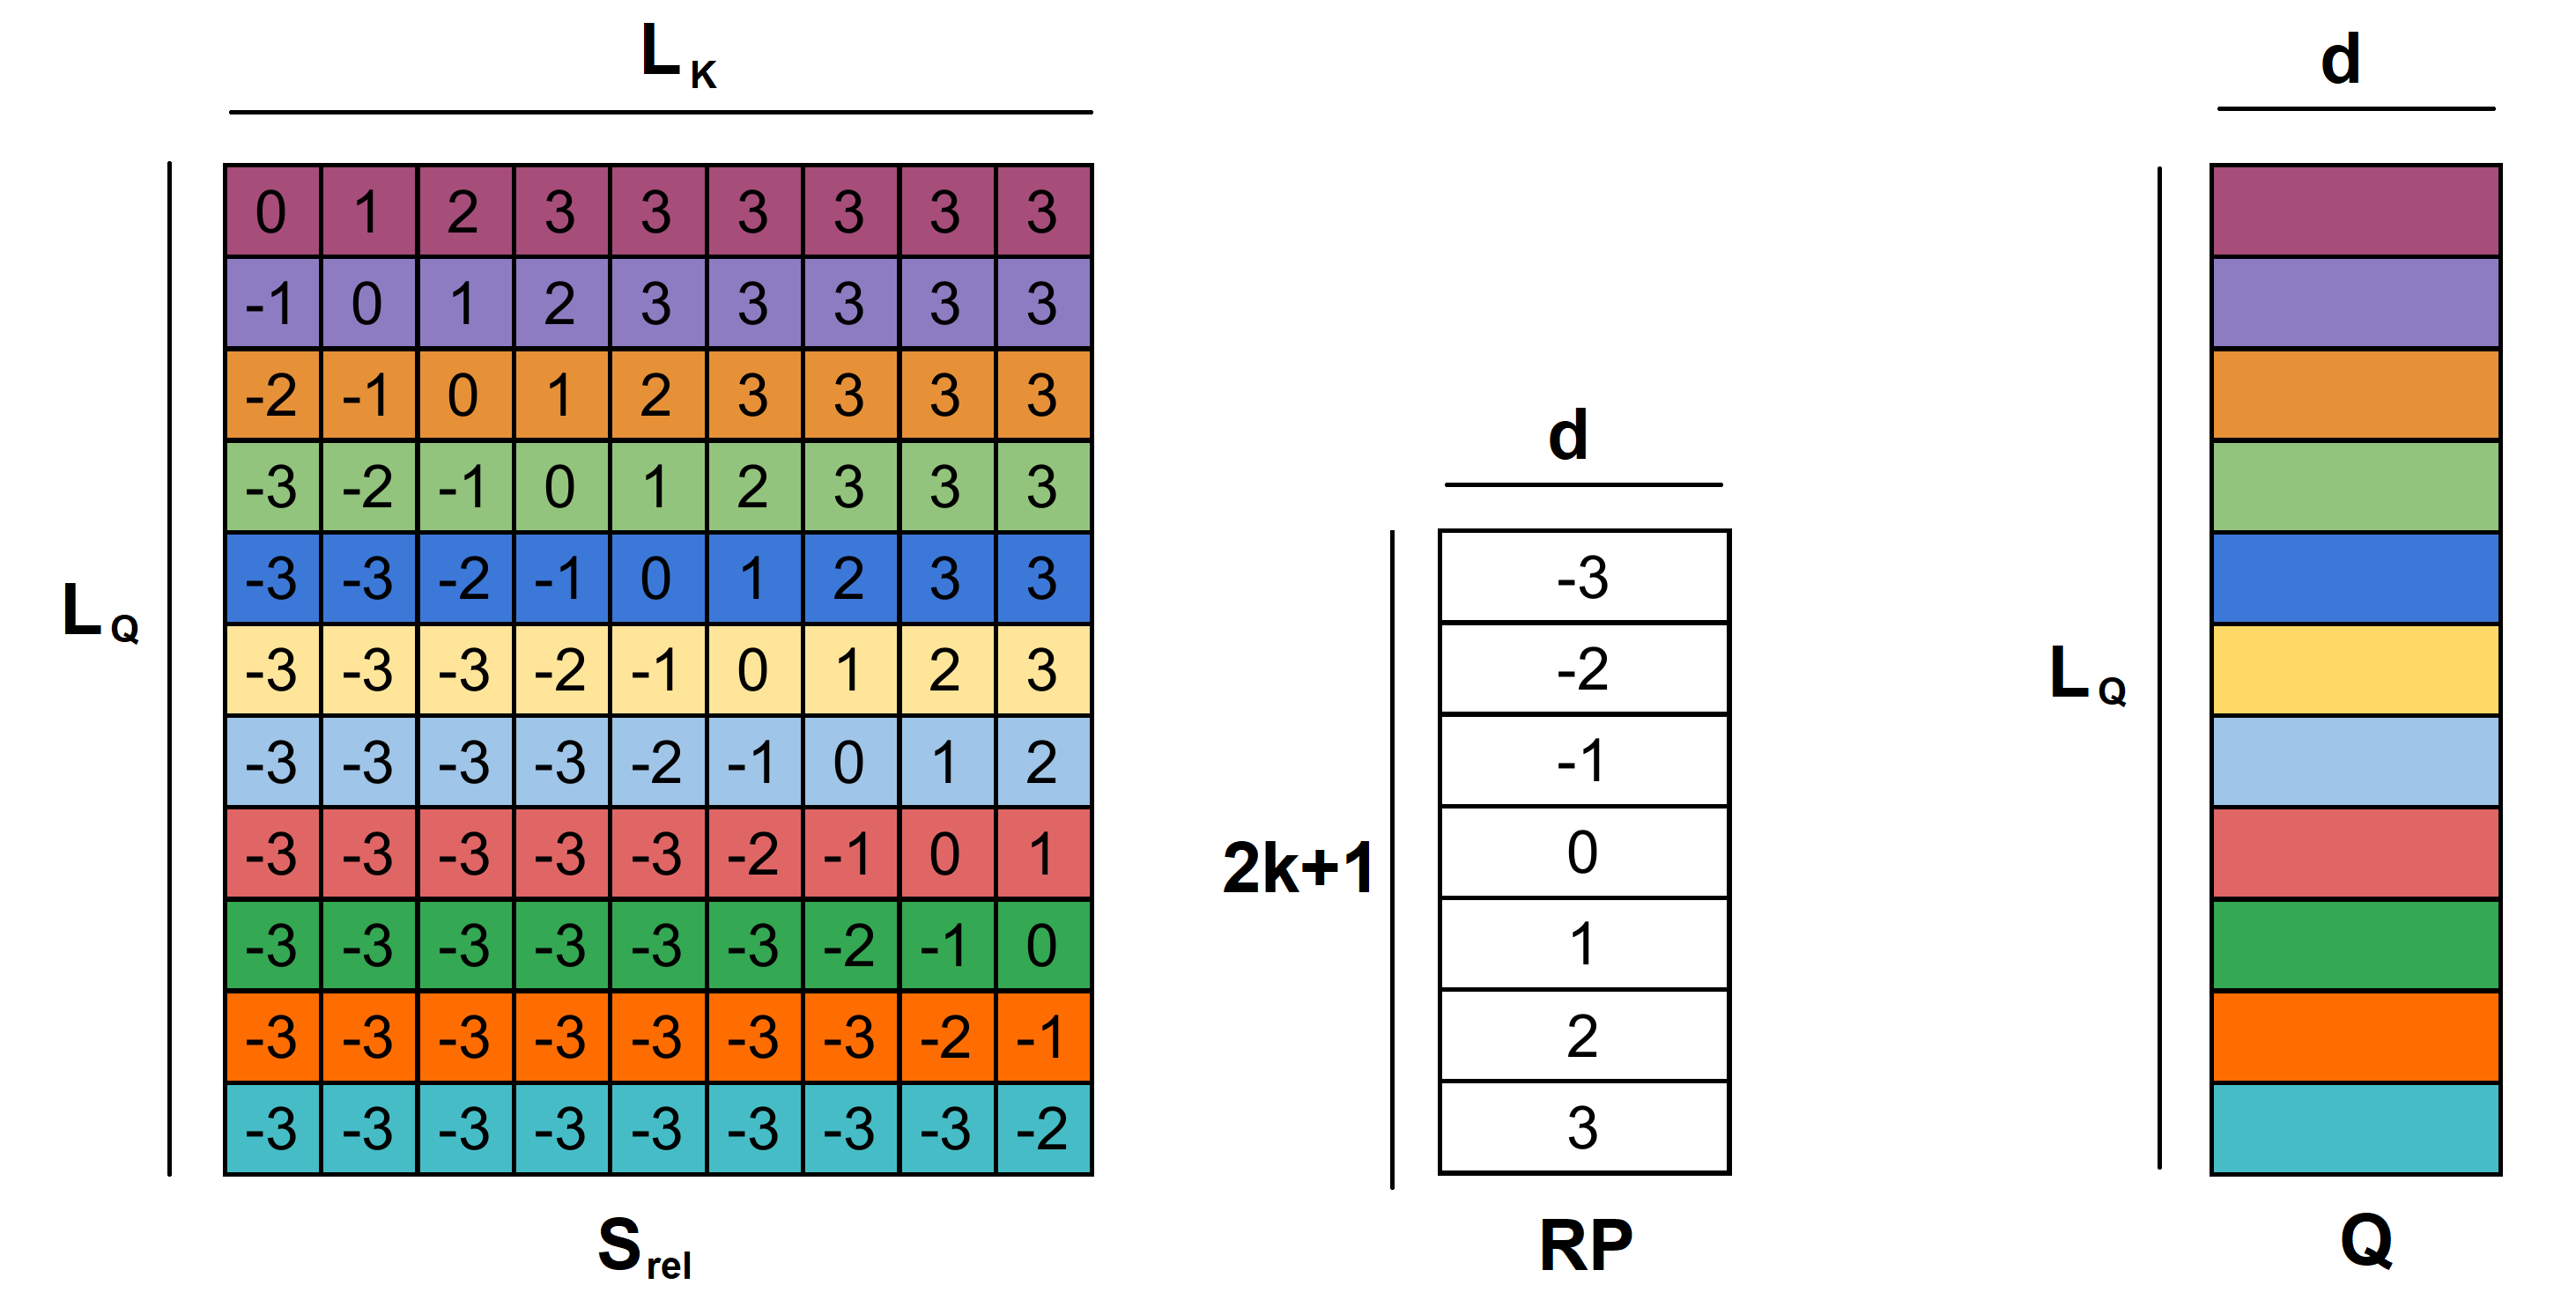
\includegraphics{images/S_rel.png}
\caption{S\_rel calculation}
\end{figure}

This score matrix must then be multiplied by the matrix of value
vectors: \(A_{rel} = S_{rel} \times V\). Each row can be interpreted as
a set of weights in the weighted sum of the value vectors.

\begin{figure}
\centering
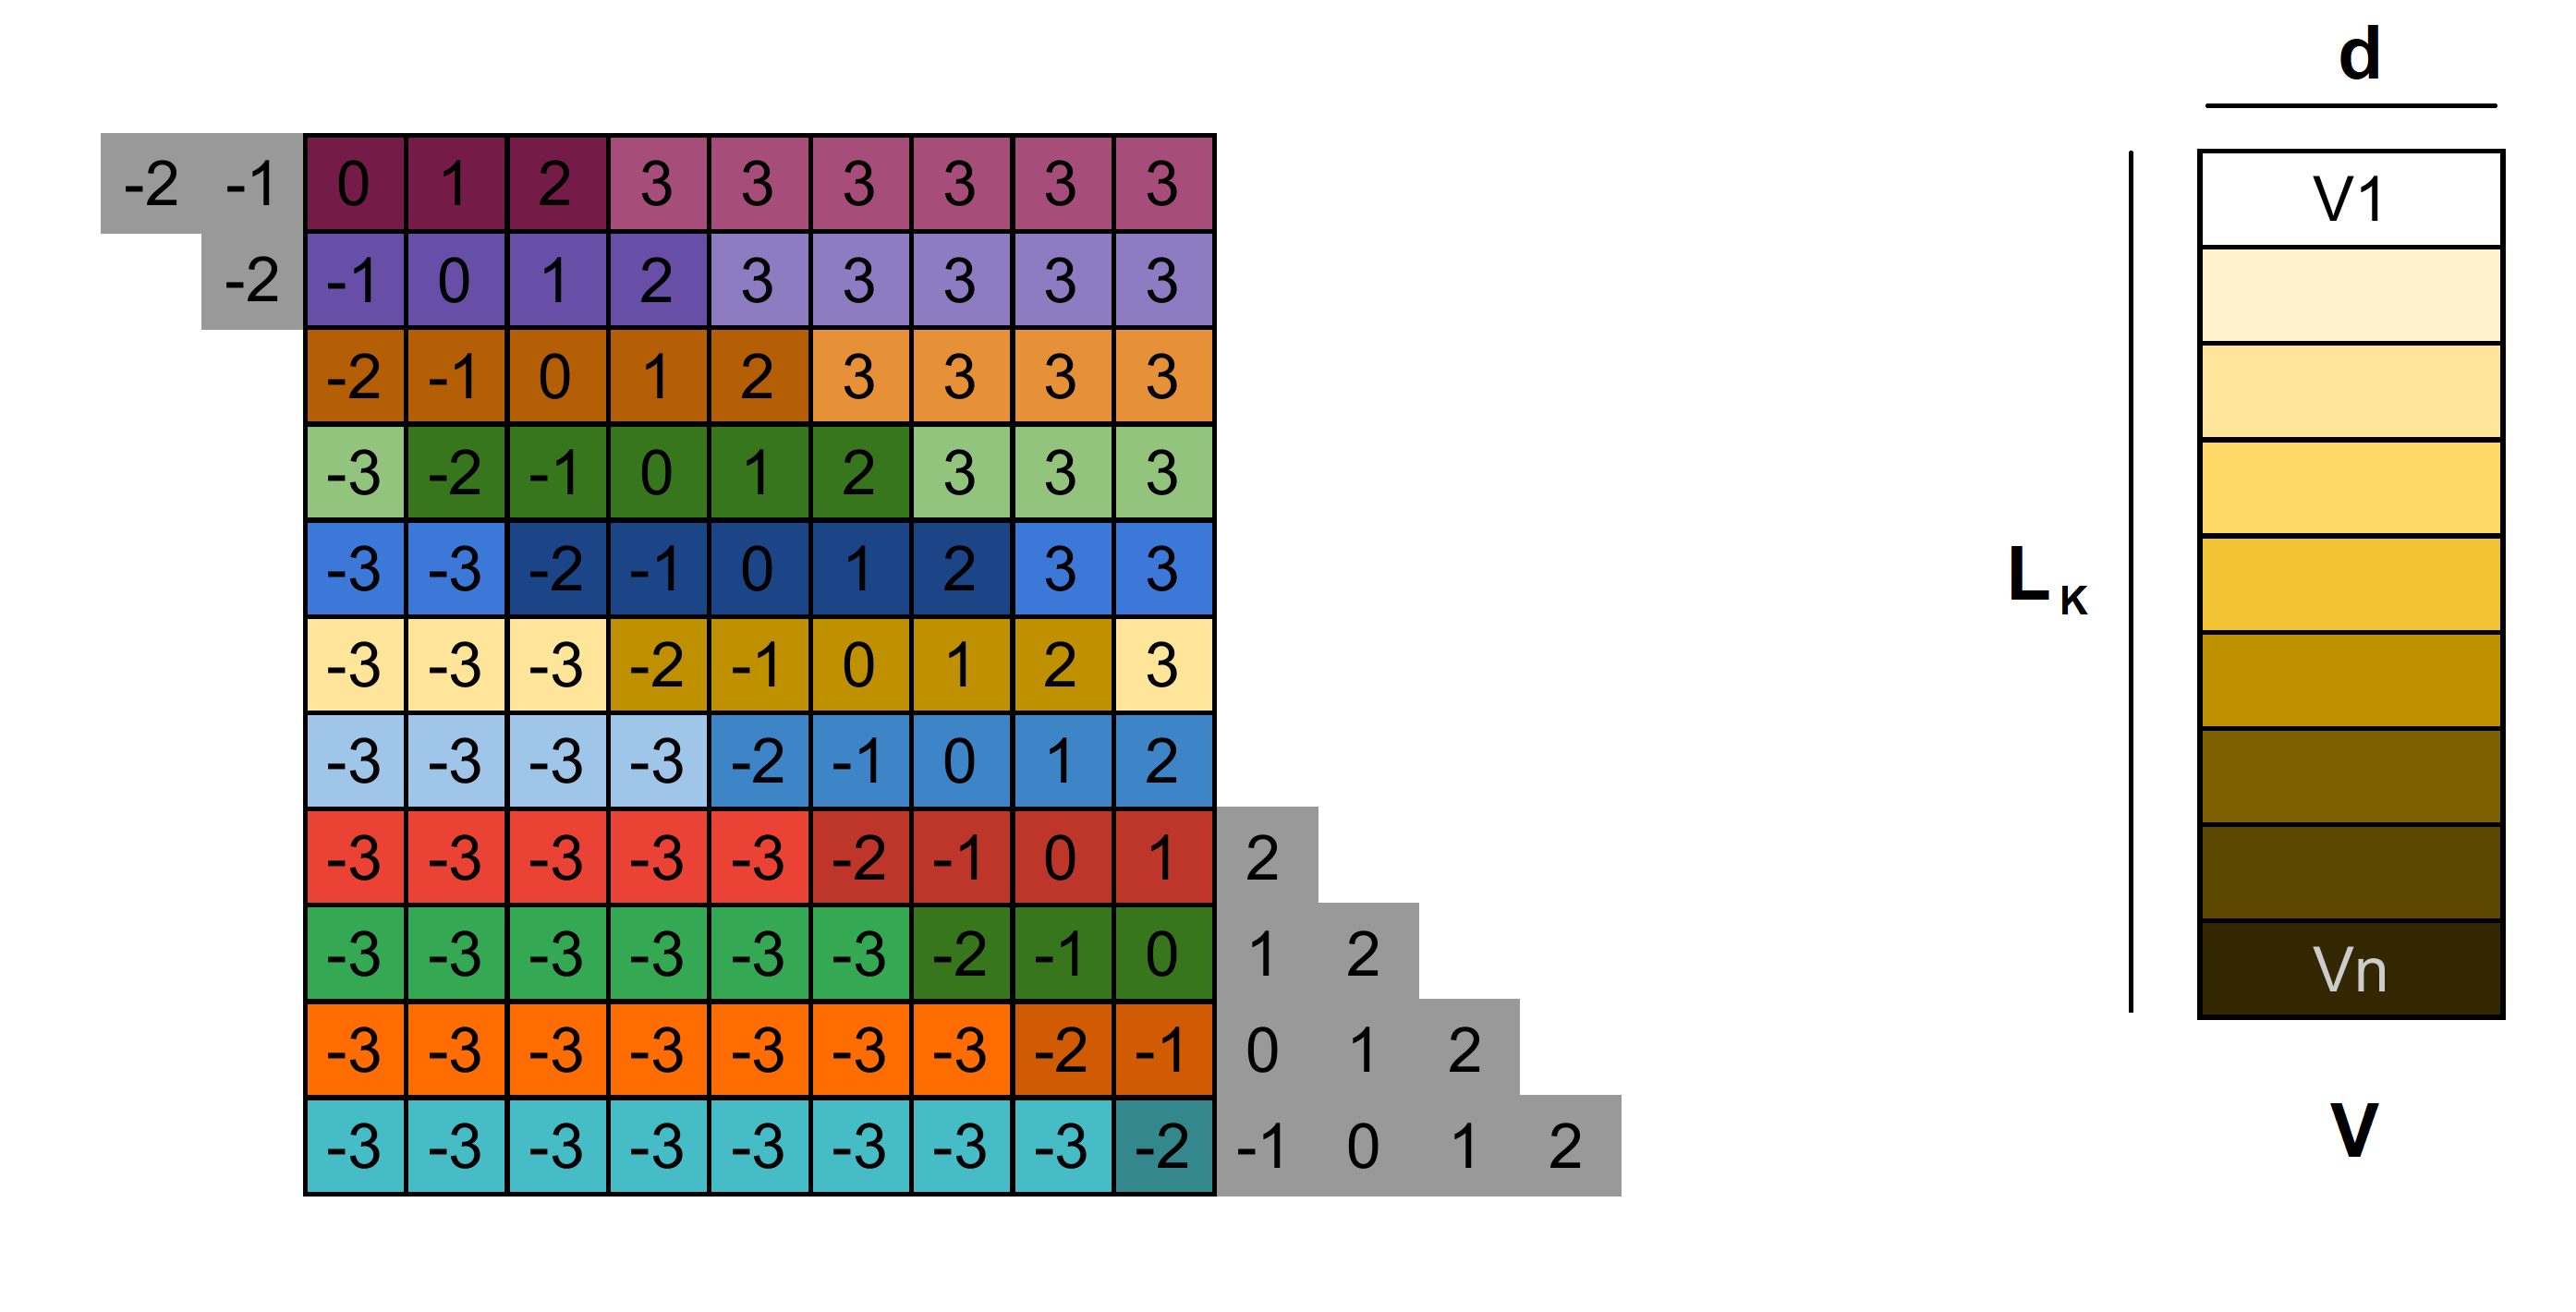
\includegraphics{images/S_rel_V.png}
\caption{A\_rel calculation}
\end{figure}

One can observe that the some weights are repeated several times in the
\(S_{rel}\) matrix. So calculating the whole matrix can be avoided by
instead calculating the dot product of each query vector with each
relative position's embedding (complexity
\(O \left(L_Q\times d\times(2k+1)\right)\)). The operation can then be
decomposed in three terms: the lower triangle, the diagonal and the
upper triangle respectively. * A set of weights that multiply a
cumulated sum of value vectors (complexity \(O(max(L_Q, L_K))\)) * A
elementwise multipliation between two tensors (complexity
\(O(L_Q\times (2k-1) \times d)\)) * A set of weights that multiply a
cumulated sum of value vectors (complexity \(O(max(L_Q, L_K))\))

\begin{figure}
\centering
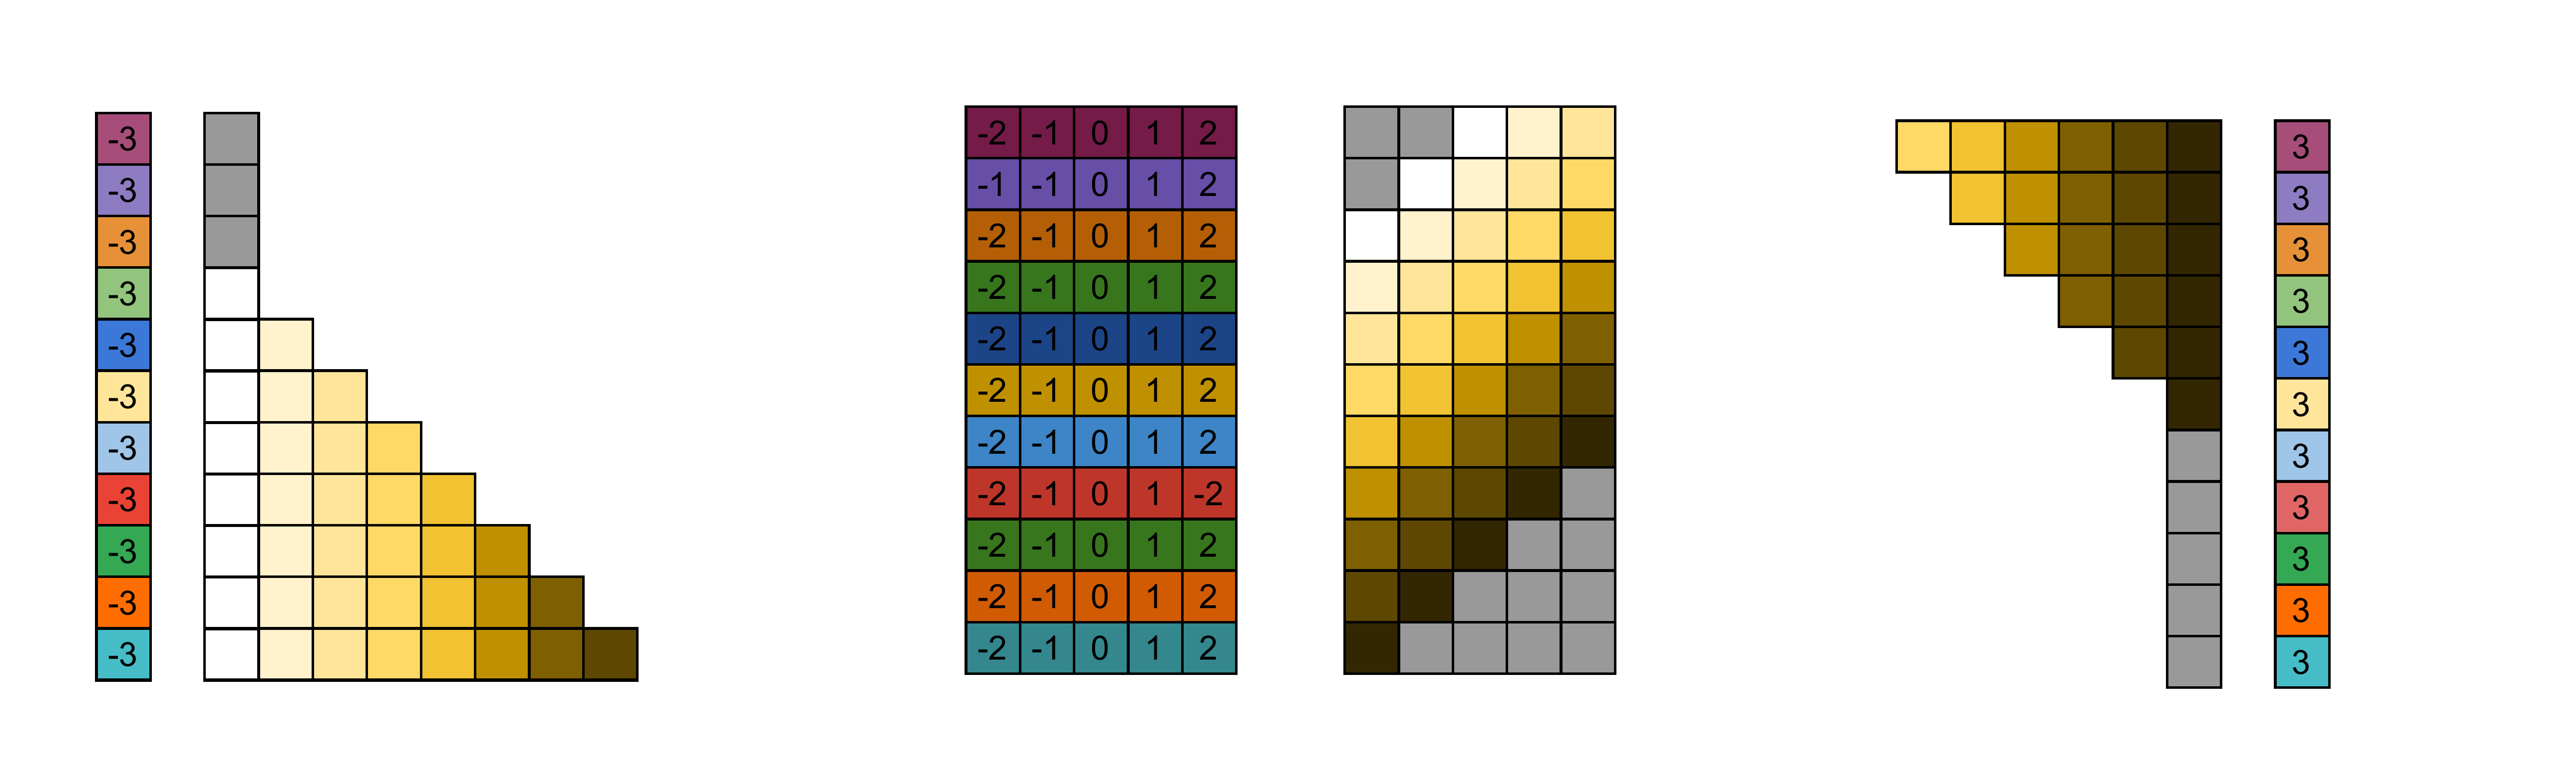
\includegraphics{images/S_rel_V_detailed.png}
\caption{A\_rel simplified calculation}
\end{figure}

Thus the attention can in fact be computed with linear complexity if we
get rid of the softmax function.

The memory used can be further reduced by observing that the right side
of the second element is a strided view of a padded copy of the value
matrix. Moving of one cell along the first dimension is equivalent to
moving along one cell of the second dimension.

The calculation can be implemented as follow, using zero-based slice
notation for compactness:

\begin{itemize}
\tightlist
\item
  \(\phi(Q)\), \(\phi(V)\) and \(RP\), are matrices of shape
  \((L_Q, d)\), \((L_K, d)\) and \((2k+1, d)\) respectively
\item
  The dot product of each query and each relative position embedding is
  calculated as \(weights = \phi(Q) \times RP^T\)
\item
  The weights of the horizon before and after are
  \(H_{before} = weights_{[:, 0]}\) and
  \(H_{after} = weights_{[:, -1]}\)
\item
  The weights of the diagonal are defined as
  \(window = weights_{[:,1:-1]}\). For the masked case, columns on the
  right of the \(k^{th}\) columns are set to 0
  (\(window_{[:, k+1:]} = 0\))
\item
  The left term is calculated as
  \(left = H_{before} * align(lower, min(max(0, L_Q-k), L_K))\) with
  \(lower\) the concatenation of:

  \begin{itemize}
  \tightlist
  \item
    a tensor of zeros of shape \(\left(min(k, L_Q), d\right)\)
  \item
    \(cumsum(V, dim=0)\)
  \end{itemize}
\item
  The middle term is calculated as \(middle = diagonal \odot strided\)
  with \(strided\) the strided view of:

  \begin{itemize}
  \tightlist
  \item
    a tensor of 0 of shape \((max(0, k-1), d)\)
  \item
    the value matrix \(V\)
  \item
    a tensor of shape \((max(0, L_Q-L_K), d)\)
  \end{itemize}
\item
  The right term is calculated as \(right = 0\) for masked case, or for
  bidirectional case, \(right = H_{right} * reverse\), with reverse the
  concatenation of:

  \begin{itemize}
  \tightlist
  \item
    a tensor of 0 of shape \((L_Q-max(0, L_K-k), d)\)
  \item
    \(sum(V_{[inf, sup]}, dim=0) - cumsum(V_{[inf, sup-1]}, dim=0)\)
    with \(inf = k-1\), \(sup = min(L_Q+k, L_K)\)
  \end{itemize}
\item
  The resulting attention function is \(A = left + middle + right\)
\end{itemize}

with:

\begin{itemize}
\tightlist
\item
  \(*\) the elementwise multiplication
\item
  \(\odot\) the elementwise multiplication followed by sum along second
  dimension
\item
  all concatenations done along the first dimension
\end{itemize}

\hypertarget{iv-linear-scalable-transformer-model}{%
\subsection{IV Linear Scalable Transformer
model}\label{iv-linear-scalable-transformer-model}}

As stated earlier, the proposed model proposes the replacement of the
scaled dot-product attention from original Transformer architecture by a
kernelized attention with relative positional encoding

The proposed model replaces the scaled-dot-product-attention by a
kernelized attention with RPE. Following the observations of
\href{https://arxiv.org/abs/1803.02155}{Shaw et al.~(2018)} that
cumulating absolute positional encoding with relative positional
encoding yield no benefits, the positional encoding is also removed -
althought for some specific applications it might be beneficial to
maintain it. The algorithm used to calculate each term is chosen
dynamically to occupy the least memory depending on the sequence lengths
and embedding dimensions - as memory usage is easier to evaluate
precisely than execution time.

In this work we have chosen the following formulation, with
\(\phi(x) = elu(x) + 1\).

\[A = \frac{\left( \phi(Q) \times \phi(K^T) + S^{rel} \right)}{\sum_j \left( \phi(Q) \times \phi(K^T) + S^{rel} \right)} \times V\]

This is essentially a combination of two terms: the kernelized attention
proposed by \href{https://arxiv.org/abs/2006.16236}{Katharopoulos et
al.~(2020)}, and the relative positional encoding proposed by
\href{https://arxiv.org/abs/1803.02155}{Shaw et al.~(2018)}. The left
term is the score matrix of shape \((L_Q, L_K)\), with a denominator
which scales all rows so that they sum to 1. For the sake of the
implementation, the multiplication must be distributed as:

\[A = \frac{\left( \phi(Q) \times \phi(K^T) \times V \right) + \left( S^{rel} \times V\right)}{\sum_j \left( \phi(Q) \times \phi(K^T) \right) + \sum_j \left( S^{rel} \right)}\]

The denominator can be easily calculated by applying the (naive or
linear complexity) algorithms with V replaced by a matrix of shape
\((L_K, 1)\) full of 1.

For each case (masked/bidirectional) the algorithm is chosen between
naive and linear complexity to occupy the least memory.

\begin{itemize}
\tightlist
\item
  for the masked \(Q \times K^T \times V\) term, the memory occupied by
  the naive algorithm is \(L_QL_K\) while the linear complexity
  algorithm occupies \(d^2 \times max(L_Q, L_K)\)
\item
  for the bidirectional \(Q \times K^T \times V\) term, the memory
  occupied by the naive algorithm is \(L_QL_K\) while the linear
  complexity algorithm occupies \(d^2\)
\item
  for the \(S_{rel} \times V\) term (masked and bidirectional), the
  memory occupied by the naive algorithm is \(L_QL_K\) while the linear
  complexity algorithm occupies \(L_Q \times (2k+1 + 4)\)
\end{itemize}

\hypertarget{v-results}{%
\subsection{V results}\label{v-results}}

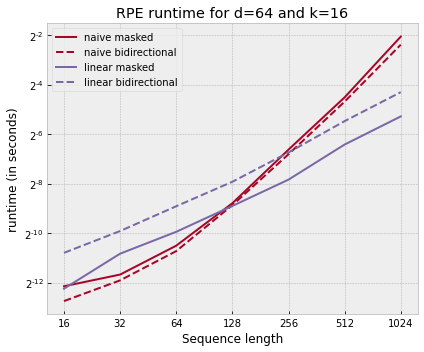
\includegraphics{images/timings/runtimes_RPE.png}

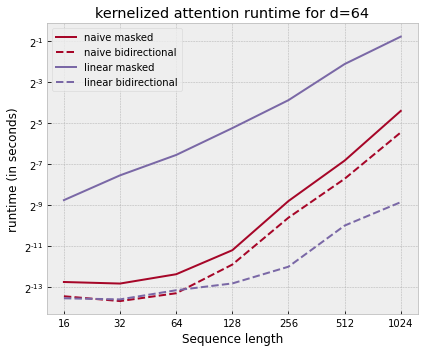
\includegraphics{images/timings/runtimes_KA.png}

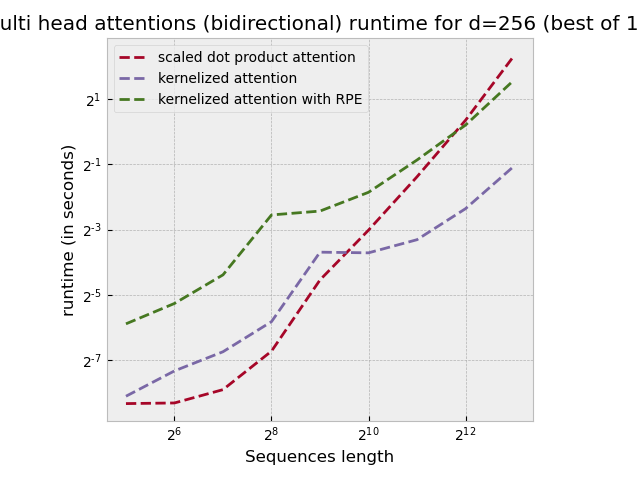
\includegraphics{images/timings/runtimes_MHA.png}

\hypertarget{conclusion}{%
\subsection{Conclusion}\label{conclusion}}

In the present work an easily implemented algorithm to compute
\href{https://arxiv.org/abs/1803.02155}{Shaw et al.~(2018)}'s relative
positional embedding with linear complexity has been presented. An
implementation of \href{https://arxiv.org/abs/2009.14794}{Choromanski et
al.~(2020)}'s prefix sum algorithm that doesn't requires custom CUDA
code (while maintaining linear complexity) was also presented.

These two elements allowed to define a kernelized attention function
with relative positional encoding, that can be computed with linear
complexity with regards to sequence length. The proposed model presents
linear scalability with sequence length, can be implemented out of the
boxe in neural network framework, and is adapted to sequence to sequence
problems instead of being restricted to encoders only models.
